\section{The Effect of Model Merging in Dense Models}
\label{app-dense}
%\subsection{Hello World}
We also conducted model merging experiments on Dense architecture models, ranging from small Seed-Dense-411M models to large Seed-Dense-70B models. Since the 411M and 2B models were not sufficiently trained, we used a configuration of N=6 for merging, with weight intervals (V) of 2B and 5B tokens, respectively. For the 8B and 70B models, which were trained more thoroughly, we used N=10, with V values of 15B and 40B for merging. As shown in Figure~\ref{fig:dense}, models of different sizes achieved significant improvements on downstream tasks after model merging. Notably, the performance gains of larger models were not smaller than those of smaller models. Specifically, Seed-Dense-70B improved from 50.6 to 57.9 on humaneval and from 85.9 to 91.3 on GSM8K. This further validates the robustness and generalization ability of \OURS{}, demonstrating that it can work across different model architectures and sizes.
\begin{figure}[h]
    \centering
    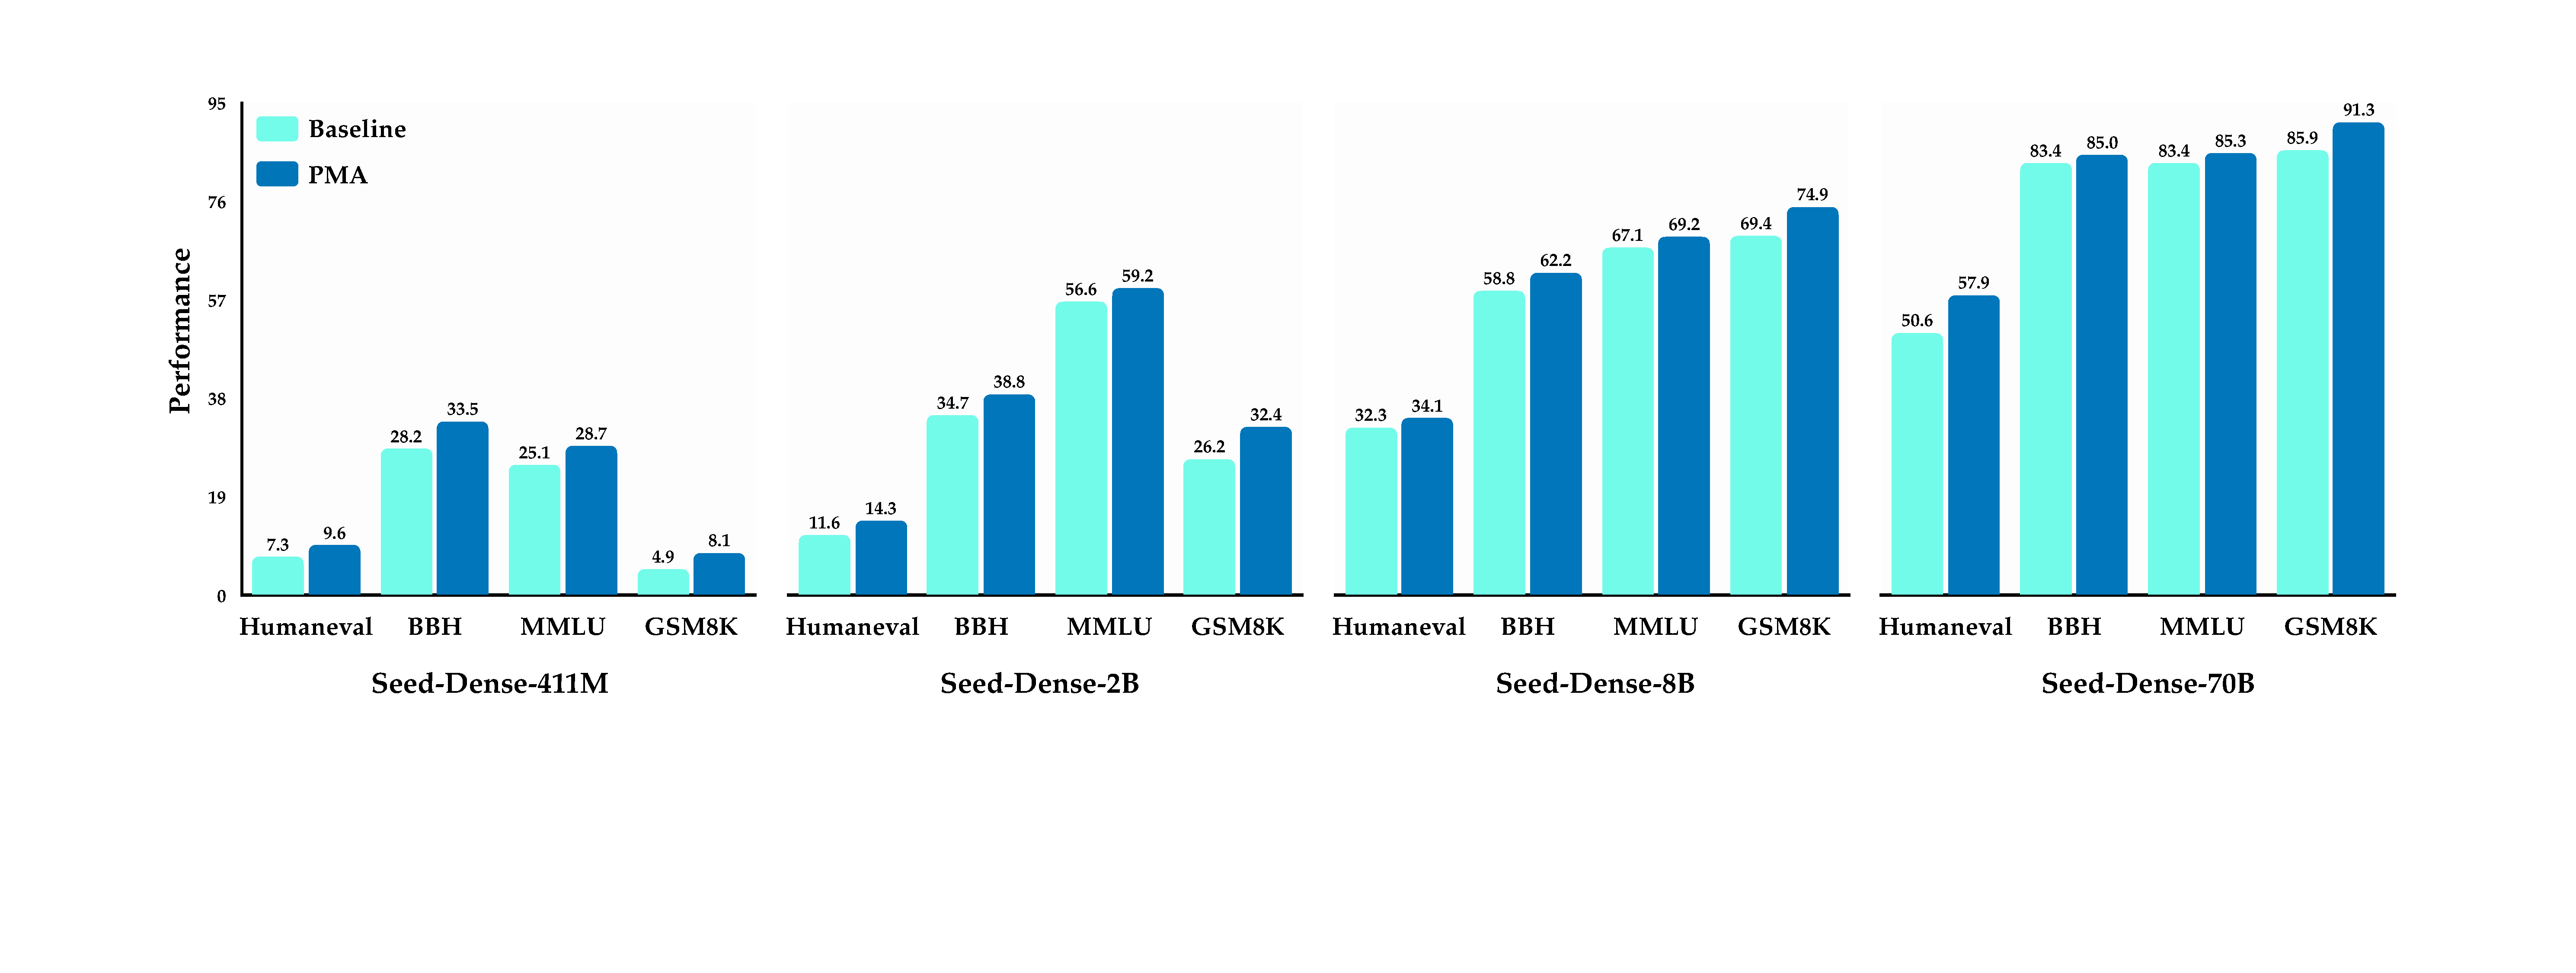
\includegraphics[width=1\linewidth]{image/dense.pdf}
    \caption{Comparison of downstream task performance for dense models of varying sizes under stable training, before
and after model merging.}
    \label{fig:dense}
\end{figure}

\section{Model Merging at the CT Stage for Supervised Fine-Tuning}
\label{app-sft}
We conducted an ablation study to assess the sensitivity of the \OURS{}-init during the SFT stage to varying learning rate schedules.
This study included experiments on merged Seed-MoE-15B/150B models following stable training on approximately 16T tokens, as well as after further training on 1T tokens with cosine annealing.
We conducted SFT training for 220M tokens using both the original weights and \OURS{}-init weights. For the original weights, we used a cosine learning rate schedule with an initial learning rate of 2e-5 and an end learning rate of 2e-6. For the \OURS{}-init weights, we used cosine schedules with initial learning rates of 1e-5, 2e-5, and 4e-5, all with an end learning rate of 2e-6. We evaluated the trained models using Open-Benchmark, which includes MMLU~\cite{hendrycks2020measuring}, LiveBench~\cite{white2024livebench}, AMC-2023, GPQA~\cite{rein2024gpqa} and LiveCodeBench~\cite{white2024livebench}, as well as our in-house evaluation set comprising OOD, Reasoning, and Instruction Following assessments.
\begin{table*}[h]
    \caption{Comparisons of performance metrics during SFT stage with varying $lr$ schedules, where a cosine scheduler is adopted to decay learning rate from $lr_{peak}$ to $lr_{end}$ (denoted as $lr_{peak} \rightarrow lr_{end}$). $\texttt{PMA}$ and $\texttt{baseline}$, stand for whether our \texttt{\OURS{}-init} technique is employed or not, respectively. IF refers to Instruction Following. }
    \centering
    \resizebox{\textwidth}{!}{
    \begin{tabular}{l|ccccc|ccc}
    \toprule				
     \multirow{2}{*}{\textbf{Model}} & \multicolumn{5}{c}{\textbf{Open-Benchmark}} & \multicolumn{3}{c}{\textbf{In-house Evaluation}} \\
     \cmidrule(lr){2-6} \cmidrule(lr){7-9}
     & \textbf{MMLU}  & \textbf{LiveBench} &  \textbf{AMC-2023} & \textbf{GPQA} & \textbf{LiveCodeBench} & \textbf{OOD} & \textbf{Reasoning} & \textbf{IF}\\
     \midrule
     \midrule
     $\textbf{Baseline}_{2e^{-5}\rightarrow 2e^{-6}}$ & 86.8 & 50.5 & 61.0 & \textbf{55.2} & \textbf{39.7} & 32.6 & 32.1 & 36.3 \\
     % \cmidrule(lr){1-1}
     $\textbf{PMA}_{2e^{-5}\rightarrow 2e^{-6}}$      & \underline{87.1} & \underline{52.0} & \underline{64.0} & 54.0 & \underline{39.4} & \textbf{34.7} & \textbf{34.0} & \textbf{38.8} \\
     $\textbf{PMA}_{1e^{-5}\rightarrow 2e^{-6}}$      & \textbf{87.2} & \textbf{53.2} & \textbf{65.5} & 54.4 & \textbf{39.7} & 33.8 & 33.2 & 37.3 \\
     $\textbf{PMA}_{4e^{-5}\rightarrow 2e^{-6}}$   &  87.0  & 51.3 & 61.4    &  54.0 & 39.2  & 31.8 & 32.6 & 37.2\\
    \bottomrule
    \end{tabular}}

    \label{sfteval}
\end{table*}
As shown in Table~\ref{sfteval}, with the same learning rate, \texttt{\OURS{}-init} significantly outperformed the baseline on both Open-Benchmark and our in-house evaluations. 
Notably, on the in-house evaluation set, we observed improvements of over two points in OOD and Instruction Following, and a 1.9-point increase in Reasoning. 
In the other two experiments with different learning rates, we also saw some degree of improvement compared to the baseline, especially with \OURS{}$_{1e^{-5}\rightarrow2e^{-6}}$, which showed gains of 2.7 points on Livebench and 4.5 points on AMC-2023.

However, we were unable to replicate such significant gains in subsequent experiments with other model sizes, although it did not negatively impact the final downstream model performance. Therefore, as a low-cost approach, \OURS{}-init is worth trying to obtain a more powerful downstream model.

\section{Limitations}
\label{limitations}
In our study, we thoroughly investigated the potential of model merging in the pre-training phase, offering significant advantages for teams working on large-scale model pre-training to pursue more daring explorations. This is due to the fact that model merging can replicate the benefits of simulated annealing, greatly shortening the exploration period during pre-training. While our experiments were extensive, certain aspects still remain open for deeper research.

In our experiments, we defaulted to using the optimal learning rate derived from the scaling law for model training, without extensively exploring the impact of learning rate on model merging. In our practice, we believe that training with a higher learning rate could lead to a better model through model merging, which aligns with the findings in \cite{sanyal2023early}. However, due to the high computational cost, we did not further quantify the impact of learning rate on model merging in a more detailed manner. 

Additionally, this paper primarily focuses on the application of model merging in pre-training. In reality, due to innovations in RL algorithms~\citep{yu2025dapo,yuan2025vapo,shao2024deepseekmath}, RL training has become more stable and often involves longer training cycles, during which a series of adjacent weights can be obtained. This paper does not investigate model merging in the context of post-training scenarios, and we leave this aspect for future research.

% \begin{table}
%     \centering
%     \begin{tabular}{cccccccccc}
%          & \multicolumn{6}{c}{Open-Benchmark} & \multicolumn{3}{c}{In-house Evaluation} \\
%          & MMLU & CEval & LiveBench & BBH & MATH & LiveCodeBench & OOD & Reasoning & Instruction Following\\
%          &  &  &  &  &  &  &  &  & \\
%          &  &  &  &  &  &  &  &  & \\
%          &  &  &  &  &  &  &  &  & \\
%          &  &  &  &  &  &  &  &  & \\
%     \end{tabular}
%     \caption{Caption}
%     \label{tab:my_label}
% \end{table}